% ============================================================
% 高考满分突破10 — 数学思想方法总结
% 编译命令：xelatex -interaction=nonstopmode 高考满分突破10_数学思想方法总结.tex
% ============================================================
\documentclass[12pt, a4paper]{ctexart}
\usepackage[margin=2.2cm]{geometry}
\usepackage{amsmath, amssymb}
\usepackage{enumitem}
\usepackage{tcolorbox}
\usepackage{booktabs}
\usepackage{array}
\usepackage{fancyhdr}
\usepackage{xcolor}
\usepackage{tikz}
\usepackage{hyperref}
\usepackage{graphicx}
\usepackage{multirow}
\usepackage{pgfplots}
\pgfplotsset{compat=1.18}

% 颜色定义
\definecolor{mainblue}{RGB}{41, 98, 168}
\definecolor{lightblue}{RGB}{230, 240, 255}
\definecolor{tipgreen}{RGB}{34, 139, 87}
\definecolor{lightgreen}{RGB}{235, 250, 240}
\definecolor{warnred}{RGB}{200, 50, 50}
\definecolor{lightred}{RGB}{255, 240, 240}
\definecolor{examorange}{RGB}{210, 120, 20}
\definecolor{lightorange}{RGB}{255, 248, 235}
\definecolor{apppurple}{RGB}{120, 60, 170}
\definecolor{lightpurple}{RGB}{245, 238, 255}

% 页眉页脚
\pagestyle{fancy}
\fancyhf{}
\fancyhead[L]{\small\textcolor{mainblue}{\textbf{高考满分突破 · 数学思想方法总结}}}
\fancyhead[R]{\small\textcolor{mainblue}{讲义10}}
\fancyfoot[C]{\small —\ \thepage\ —}
\renewcommand{\headrulewidth}{0.6pt}
\renewcommand{\headrule}{\hbox to\headwidth{\color{mainblue}\leaders\hrule height \headrulewidth\hfill}}
\renewcommand{\footrulewidth}{0pt}

% tcolorbox 样式
\newtcolorbox{knowledgebox}[1][]{%
  colback=lightblue, colframe=mainblue,
  fonttitle=\bfseries\large, title=#1,
  arc=3mm, boxrule=0.8pt,
  left=8pt, right=8pt, top=6pt, bottom=6pt
}

\newtcolorbox{tipbox}[1][]{%
  colback=lightgreen, colframe=tipgreen,
  fonttitle=\bfseries, title=#1,
  arc=2mm, boxrule=0.6pt,
  left=6pt, right=6pt, top=4pt, bottom=4pt
}

\newtcolorbox{warnbox}[1][]{%
  colback=lightred, colframe=warnred,
  fonttitle=\bfseries, title=#1,
  arc=2mm, boxrule=0.6pt,
  left=6pt, right=6pt, top=4pt, bottom=4pt
}

\newtcolorbox{examplebox}[1][]{%
  colback=lightorange, colframe=examorange,
  fonttitle=\bfseries, title=#1,
  arc=3mm, boxrule=0.8pt,
  left=8pt, right=8pt, top=6pt, bottom=6pt
}

\newtcolorbox{appbox}[1][]{%
  colback=lightpurple, colframe=apppurple,
  fonttitle=\bfseries, title=#1,
  arc=3mm, boxrule=0.8pt,
  left=8pt, right=8pt, top=6pt, bottom=6pt
}

\setCJKmainfont{Hiragino Sans GB}
\setCJKsansfont{Heiti SC}

\begin{document}

% ============ 标题页 ============
\begin{center}
{\Huge\bfseries\textcolor{mainblue}{高考数学满分突破}}\\[6pt]
{\LARGE\bfseries\textcolor{mainblue}{数学思想方法总结}}\\[12pt]
\rule{0.6\textwidth}{1pt}\\[8pt]
{\normalsize 适用：高三冲刺\quad |\quad 课时：2课时}
\end{center}
\vspace{10pt}

% ============================================================
%  第一部分：知识点讲解
% ============================================================
\section*{\textcolor{mainblue}{一、知识点讲解}}

% —— 1.1 化归与转化 ——
\subsection*{1.1\quad 化归与转化}

\begin{knowledgebox}[化归与转化思想]
化归与转化是数学中最基本、最核心的思想方法，其本质是：\textbf{将未知问题转化为已知问题，将复杂问题转化为简单问题}。

常见的化归方向：
\begin{enumerate}[label=(\arabic*)]
  \item \textbf{高次化低次}：利用换元、因式分解等手段降幂。
  \item \textbf{多元化一元}：通过消元、代入减少变量。
  \item \textbf{陌生化熟悉}：将新情境问题化归为已知模型（如将向量问题化为坐标运算）。
  \item \textbf{数与形互化}：代数问题用几何直观，几何问题用代数精确计算。
  \item \textbf{一般与特殊互化}：先用特殊值猜想，再一般化证明；或先研究一般规律，再处理特殊情况。
\end{enumerate}
\end{knowledgebox}

\begin{tipbox}[化归的三个层次]
\begin{enumerate}[label=\textbf{第\arabic*层}]
  \item \textbf{等价转化}：变形前后完全等价（如方程的同解变形），无增根无失根。
  \item \textbf{充分/必要转化}：$A\Rightarrow B$ 则 $B$ 的解需回代验证（如不等式两边平方可能引入增解）。
  \item \textbf{构造转化}：构造辅助函数、辅助图形，将问题嵌入更大的框架中求解。
\end{enumerate}
\end{tipbox}

% —— 1.2 数形结合高观点 ——
\subsection*{1.2\quad 数形结合高观点}

\begin{knowledgebox}[数形结合思想]
数形结合的核心：\textbf{以形助数，以数解形}。
\begin{enumerate}[label=(\arabic*)]
  \item \textbf{以形助数}：将代数式、方程、不等式赋予几何意义，借助图形的直观性快速获得解题方向。
  \item \textbf{以数解形}：将几何图形坐标化、向量化、参数化，用代数方法精确求解。
\end{enumerate}
\end{knowledgebox}

\begin{tipbox[高考高频数形结合场景]
\begin{enumerate}[label=(\arabic*)]
  \item 函数零点问题 $\longleftrightarrow$ 两函数图像交点。
  \item 不等式 $f(x)>g(x)$ $\longleftrightarrow$ 函数图像的上下位置关系。
  \item 向量运算 $\longleftrightarrow$ 平行四边形、三角形。
  \item 线性规划 $\longleftrightarrow$ 可行域与目标函数截距。
  \item 复数运算 $\longleftrightarrow$ 复平面上的旋转与伸缩。
  \item 方程 $|x-a|+|x-b|=c$ $\longleftrightarrow$ 数轴上距离之和。
  \item 圆锥曲线定义 $\longleftrightarrow$ 焦点与准线的距离关系。
\end{enumerate}
\end{tipbox}

% —— 1.3 分类讨论逻辑结构 ——
\subsection*{1.3\quad 分类讨论的逻辑结构}

\begin{knowledgebox}[分类讨论思想]
当问题的条件或结论在不同情况下有不同的表现时，需要\textbf{不重不漏}地进行分类讨论。

分类讨论的标准：
\begin{enumerate}[label=(\arabic*)]
  \item \textbf{由数学概念引起}：绝对值的正负、对数的底数范围、二次项系数是否为零。
  \item \textbf{由运算法则引起}：不等式两边乘以负数需变号、等比数列公比 $q=1$ 与 $q\neq 1$。
  \item \textbf{由图形位置引起}：点在直线的哪一侧、直线与圆的位置关系。
  \item \textbf{由参数范围引起}：含参问题中参数的不同取值导致不同结果。
\end{enumerate}
\end{knowledgebox}

\begin{warnbox}[分类讨论的常见错误]
\begin{enumerate}[label=(\arabic*)]
  \item \textbf{分类不全}：遗漏某种情况（如忘记讨论二次项系数为零）。
  \item \textbf{分类重叠}：同一情况被讨论两次，导致重复计算。
  \item \textbf{结论不统一}：各分支的结论应合并为最终答案，不能"各说各话"。
  \item \textbf{讨论顺序混乱}：建议按"先主后次"的原则，先讨论最主要、最核心的分类标准。
\end{enumerate}
\end{warnbox}

% —— 1.4 满分答题策略 ——
\subsection*{1.4\quad 满分答题策略}

\begin{knowledgebox}[高考数学答题策略]
\textbf{时间分配（150分钟 / 150分）：}
\begin{itemize}
  \item 选择题+填空题：$\leq 50$ 分钟（每题平均 $2\sim3$ 分钟）。
  \item 解答题前4题：$\leq 40$ 分钟（每题约 $8\sim10$ 分钟）。
  \item 解答题后2题：$\leq 50$ 分钟（压轴题可多分配时间）。
  \item 检查：$\geq 10$ 分钟。
\end{itemize}
\end{knowledgebox}

\begin{tipbox}[答题规范要点]
\begin{enumerate}[label=(\arabic*)]
  \item \textbf{选择题策略}：排除法、特值法、数形结合法并用，不要死算。遇到难题先跳过，最后集中处理。
  \item \textbf{填空题策略}：注意单位、定义域、取值范围，答案要化简到最简形式。
  \item \textbf{解答题策略}：
    \begin{itemize}
      \item 第一步写"解："或"证明："，条理清晰。
      \item 关键步骤必须写出，不能跳步（如"由题意得"后直接写结论）。
      \item 涉及分类讨论时，先写出分类标准，再逐一讨论，最后汇总。
      \item 最后写"综上所述"或"$\therefore$"引出结论。
    \end{itemize}
  \item \textbf{检查要点}：回代验证、端点值检验、单位一致性、正负号。
\end{enumerate}
\end{tipbox}

\begin{warnbox}[满分卷面要求]
\begin{enumerate}[label=(\arabic*)]
  \item 字迹工整，卷面整洁，不要涂改过多。
  \item 解答题分步书写，不要用一个大等式从头写到尾。
  \item 关键结论用方框框出（如 $\boxed{x=3}$），方便阅卷老师快速定位。
  \item 坐标系、函数图像要画清楚，标明关键点坐标。
\end{enumerate}
\end{warnbox}

% ============================================================
%  第二部分：例题精讲
% ============================================================
\section*{\textcolor{examorange}{二、例题精讲}}

\begin{examplebox}[【例题1】化归思想——换元降幂]
解方程：$x^4 - 5x^2 + 4 = 0$。
\end{examplebox}

\textbf{解：}
令 $t = x^2$（$t\geq 0$），原方程化为
\[
  t^2 - 5t + 4 = 0 \implies (t-1)(t-4) = 0
\]
$t=1$ 时 $x=\pm 1$；$t=4$ 时 $x=\pm 2$。

\[
  \boxed{x \in \{-2,\,-1,\,1,\,2\}}
\]

\begin{tipbox}[方法总结]
高次方程的化归策略：换元降幂 $\to$ 因式分解 $\to$ 回代求解。此法可推广至 $x^6+ax^3+b=0$ 等可化为二次型的方程。
\end{tipbox}

\begin{examplebox}[【例题2】数形结合——零点个数]
判断函数 $f(x) = e^x - 2x$ 在 $(0,+\infty)$ 上零点的个数。
\end{examplebox}

\textbf{解：}
$f(x)=0 \iff e^x = 2x$。令 $y_1 = e^x$，$y_2 = 2x$，在同一坐标系中画出两条曲线。

\begin{center}
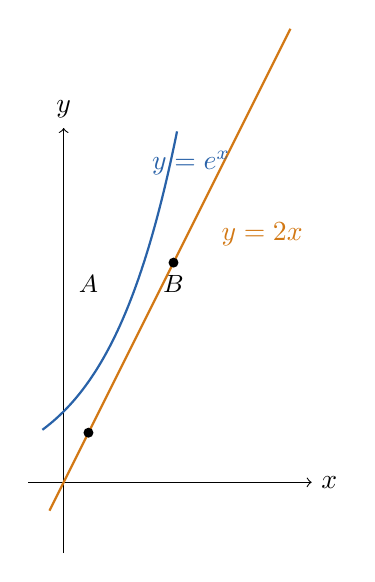
\begin{tikzpicture}[scale=0.9]
  \draw[->] (-0.5,0)--(3.5,0) node[right]{$x$};
  \draw[->] (0,-1)--(0,5) node[above]{$y$};
  \draw[thick, mainblue, domain=-0.3:1.6, samples=80] plot(\x, {exp(\x)});
  \draw[thick, examorange, domain=-0.2:3.2] plot(\x, 2*\x);
  \node[mainblue] at (1.8,4.5) {$y=e^x$};
  \node[examorange] at (2.8,3.5) {$y=2x$};
  \node at (0.35,2.8) {\small$A$};
  \node at (1.55,2.8) {\small$B$};
  \fill (0.35, 0.7) circle(2pt);
  \fill (1.55, 3.1) circle(2pt);
\end{tikzpicture}
\end{center}

分析：$f(0)=1>0$，$f(1)=e-2\approx 0.72>0$，$f(2)=e^2-4\approx 3.39>0$，但 $f(0.1)\approx 0.905>0$，$f(0.5)\approx 0.649>0$。

更精确地：$f'(x) = e^x - 2$，令 $f'(x)=0$ 得 $x=\ln 2\approx 0.693$。
$f(\ln 2) = 2 - 2\ln 2 \approx 0.614 > 0$。

$f(0) = 1 > 0$，且 $\lim_{x\to+\infty}f(x) = +\infty$，最小值 $f(\ln 2)>0$。

因此 $f(x)>0$ 恒成立，$f(x)$ 在 $(0,+\infty)$ 上\textbf{无零点}。$\boxed{0\text{ 个零点}}$

\begin{examplebox}[【例题3】分类讨论——含参二次函数]
设函数 $f(x) = ax^2 + (2a-1)x - 3$ 在 $[-1,1]$ 上的最大值为 $1$，求 $a$ 的值。
\end{examplebox}

\textbf{解：}
\textbf{情形一：} $a=0$。$f(x)=-x-3$，在 $[-1,1]$ 上为减函数，最大值 $f(-1)=-2\neq 1$，不合。

\textbf{情形二：} $a\neq 0$。$f(x)$ 是二次函数，对称轴 $x_0 = -\dfrac{2a-1}{2a} = \dfrac{1-2a}{2a}$。

\textbf{（i）} 若 $a>0$，开口向上，最大值在端点取得。
\begin{itemize}
  \item $f(-1) = a-(2a-1)-3 = -a-2$。
  \item $f(1) = a+(2a-1)-3 = 3a-4$。
\end{itemize}
$f(-1)=1 \implies a=-3<0$（舍）；$f(1)=1 \implies a=\dfrac{5}{3}$。

验证：$a=\frac{5}{3}$ 时，对称轴 $x_0 = \frac{1-10/3}{10/3} = -\frac{7}{10}\in[-1,1]$，$f(-7/10) = \frac{5}{3}\cdot\frac{49}{100}+\left(\frac{10}{3}-1\right)\left(-\frac{7}{10}\right)-3 = \frac{49}{60}-\frac{49}{30}-3 < 1$，最大值确为 $f(1)=1$。$\checkmark$

\textbf{（ii）} 若 $a<0$，开口向下，最大值在对称轴或端点取得。
$f(-1)=1 \implies a=-3$；$f(1)=1 \implies a=\frac{5}{3}>0$（舍）。

$a=-3$ 时，对称轴 $x_0 = \frac{1+6}{-6} = -\frac{7}{6} < -1$，在 $[-1,1]$ 上 $f$ 递减，最大值 $f(-1)=-(-3)-2=1$。$\checkmark$

综上，$\boxed{a=\dfrac{5}{3} \text{ 或 } a=-3}$。

\begin{examplebox}[【例题4】化归+数形结合——恒成立问题]
若不等式 $x^2 + ax + 1 \geq 0$ 对一切 $x\in[1,+\infty)$ 恒成立，求 $a$ 的取值范围。
\end{examplebox}

\textbf{解：}
$x\geq 1$ 时 $x>0$，原不等式等价于
\[
  a \geq -\frac{x^2+1}{x} = -x - \frac{1}{x}
\]
令 $g(x) = -x-\dfrac{1}{x}$（$x\geq 1$），则 $a\geq g(x)_{\max}$。

$g'(x) = -1+\dfrac{1}{x^2} < 0$（$x\geq 1$），$g$ 在 $[1,+\infty)$ 上单调递减。

$g(x)_{\max} = g(1) = -2$。

所以 $\boxed{a \geq -2}$。

\begin{examplebox}[【例题5】转化与构造——不等式证明]
已知 $a,b,c>0$ 且 $a+b+c=1$，证明：$\dfrac{1}{a}+\dfrac{1}{b}+\dfrac{1}{c}\geq 9$。
\end{examplebox}

\textbf{解：}
构造转化：由柯西不等式（或均值不等式链）：
\[
  \frac{1}{a}+\frac{1}{b}+\frac{1}{c} = \frac{(a+b+c)}{1}\cdot\left(\frac{1}{a}+\frac{1}{b}+\frac{1}{c}\right)
  \geq \frac{(1+1+1)^2}{a+b+c} = \frac{9}{1} = 9
\]
（此处使用柯西不等式：$\left(\sum\frac{1}{a}\right)\left(\sum a\right)\geq\left(\sum 1\right)^2=9$。）

等号成立当且仅当 $a=b=c=\dfrac{1}{3}$。$\blacksquare$

\begin{examplebox}[【例题6】分类讨论——绝对值不等式]
解不等式 $|2x-1|+|x+2|<5$。
\end{examplebox}

\textbf{解：}
零点为 $x=\dfrac{1}{2}$ 和 $x=-2$，分三段讨论：

\textbf{（i）} $x<-2$：$-(2x-1)-(x+2)<5 \implies -3x-1<5 \implies x>-2$。与 $x<-2$ 矛盾，无解。

\textbf{（ii）} $-2\leq x<\dfrac{1}{2}$：$-(2x-1)+(x+2)<5 \implies -x+3<5 \implies x>-2$。解为 $(-2,\frac{1}{2})$。

\textbf{（iii）} $x\geq\dfrac{1}{2}$：$(2x-1)+(x+2)<5 \implies 3x+1<5 \implies x<\dfrac{4}{3}$。解为 $[\frac{1}{2},\frac{4}{3})$。

综上，$\boxed{x\in\left(-2,\,\dfrac{4}{3}\right)}$。

\begin{examplebox}[【例题7】数形结合——向量与几何]
在 $\triangle ABC$ 中，$D$ 为 $BC$ 中点，$\overrightarrow{AB}=\mathbf{a}$，$\overrightarrow{AC}=\mathbf{b}$。用 $\mathbf{a},\mathbf{b}$ 表示 $\overrightarrow{AD}$，并证明 $|\mathbf{a}|^2+|\mathbf{b}|^2 = 2|\overrightarrow{AD}|^2 + \dfrac{1}{2}|\mathbf{a}-\mathbf{b}|^2$（中线长公式）。
\end{examplebox}

\textbf{解：}
$\overrightarrow{AD} = \overrightarrow{AB}+\overrightarrow{BD} = \mathbf{a}+\dfrac{1}{2}(\mathbf{b}-\mathbf{a}) = \dfrac{\mathbf{a}+\mathbf{b}}{2}$。

设 $\overrightarrow{AD}=\mathbf{m}=\dfrac{\mathbf{a}+\mathbf{b}}{2}$，$\overrightarrow{BC}=\mathbf{b}-\mathbf{a}$。
\begin{align*}
  2|\mathbf{m}|^2 + \frac{1}{2}|\mathbf{b}-\mathbf{a}|^2
  &= 2\cdot\frac{|\mathbf{a}+\mathbf{b}|^2}{4} + \frac{|\mathbf{b}-\mathbf{a}|^2}{2} \\
  &= \frac{|\mathbf{a}|^2+2\mathbf{a}\cdot\mathbf{b}+|\mathbf{b}|^2}{2} + \frac{|\mathbf{a}|^2-2\mathbf{a}\cdot\mathbf{b}+|\mathbf{b}|^2}{2} \\
  &= \frac{2|\mathbf{a}|^2+2|\mathbf{b}|^2}{2} = |\mathbf{a}|^2+|\mathbf{b}|^2 \qquad\blacksquare
\end{align*}

\begin{examplebox}[【例题8】化归——数列求和]
求数列 $\displaystyle a_n = \frac{1}{n(n+1)(n+2)}$ 的前 $n$ 项和 $S_n$。
\end{examplebox}

\textbf{解：}
裂项化归：
\[
  a_n = \frac{1}{n(n+1)(n+2)} = \frac{1}{2}\left[\frac{1}{n(n+1)}-\frac{1}{(n+1)(n+2)}\right]
\]
\[
  S_n = \frac{1}{2}\sum_{k=1}^{n}\left[\frac{1}{k(k+1)}-\frac{1}{(k+1)(k+2)}\right]
\]
Telescoping:
\[
  S_n = \frac{1}{2}\left[\frac{1}{1\cdot 2}-\frac{1}{(n+1)(n+2)}\right]
  = \boxed{\frac{1}{4}-\frac{1}{2(n+1)(n+2)}}
\]

\begin{examplebox}[【例题9】综合——导数与分类讨论]
设 $f(x) = x^3 - 3ax + 2$（$a\in\mathbb{R}$），讨论 $f(x)$ 的极值情况。
\end{examplebox}

\textbf{解：}
$f'(x) = 3x^2 - 3a = 3(x^2-a)$。

\textbf{情形一：} $a<0$。$f'(x) = 3(x^2-a) > 0$ 恒成立，$f$ 在 $\mathbb{R}$ 上单调递增，\textbf{无极值}。

\textbf{情形二：} $a=0$。$f'(x)=3x^2\geq 0$，等号仅在 $x=0$ 时成立，$f$ 单调递增，\textbf{无极值}。

\textbf{情形三：} $a>0$。$f'(x)=0$ 的两根为 $x=\pm\sqrt{a}$。
\begin{itemize}
  \item $x<-\sqrt{a}$ 时 $f'>0$（递增）。
  \item $-\sqrt{a}<x<\sqrt{a}$ 时 $f'<0$（递减）。
  \item $x>\sqrt{a}$ 时 $f'>0$（递增）。
\end{itemize}
$x=-\sqrt{a}$ 为极大值点，极大值 $f(-\sqrt{a}) = -a\sqrt{a}+3a\sqrt{a}+2 = 2a\sqrt{a}+2$。\\
$x=\sqrt{a}$ 为极小值点，极小值 $f(\sqrt{a}) = a\sqrt{a}-3a\sqrt{a}+2 = -2a\sqrt{a}+2$。

\begin{examplebox}[【例题10】满分答题示范——圆锥曲线]
已知椭圆 $\dfrac{x^2}{4}+\dfrac{y^2}{3}=1$，$F_1,F_2$ 为左、右焦点，过 $F_2$ 的直线 $l$ 交椭圆于 $A,B$ 两点，求 $\triangle F_1AB$ 面积的最大值。
\end{examplebox}

\textbf{解：}
$a=2,\,b=\sqrt{3},\,c=1$，$F_1(-1,0)$，$F_2(1,0)$。

设 $l$ 的方程为 $x = my+1$（这样可以涵盖所有过 $F_2$ 的直线，避免讨论斜率不存在）。

代入椭圆方程：$\dfrac{(my+1)^2}{4}+\dfrac{y^2}{3}=1$，化简：
\[
  3m^2y^2+6my+3+4y^2 = 12
\]
\[
  (3m^2+4)y^2+6my-9 = 0
\]
设 $A(x_1,y_1),\,B(x_2,y_2)$，则 $y_1+y_2=\dfrac{-6m}{3m^2+4}$，$y_1 y_2=\dfrac{-9}{3m^2+4}$。

$\triangle F_1AB$ 的面积：
\[
  S = \frac{1}{2}|F_1F_2|\cdot|y_1-y_2| = \frac{1}{2}\cdot 2\cdot|y_1-y_2| = |y_1-y_2|
\]
\[
  |y_1-y_2|^2 = (y_1+y_2)^2-4y_1y_2 = \frac{36m^2}{(3m^2+4)^2}+\frac{36}{3m^2+4} = \frac{36(m^2+1)+36m^2}{(3m^2+4)^2}\cdot\frac{3m^2+4}{1}
\]
Wait, let me recompute:
\[
  |y_1-y_2|^2 = \frac{36m^2}{(3m^2+4)^2}+\frac{36(3m^2+4)}{(3m^2+4)^2} = \frac{36m^2+108m^2+144}{(3m^2+4)^2} = \frac{144(m^2+1)}{(3m^2+4)^2}
\]
\[
  S = |y_1-y_2| = \frac{12\sqrt{m^2+1}}{3m^2+4}
\]
令 $t = m^2+1\geq 1$，则 $3m^2+4 = 3t+1$：
\[
  S = \frac{12\sqrt{t}}{3t+1}
\]
令 $g(t) = \dfrac{12\sqrt{t}}{3t+1}$（$t\geq 1$）。

$g'(t) = 12\cdot\dfrac{\frac{1}{2\sqrt{t}}(3t+1)-\sqrt{t}\cdot 3}{(3t+1)^2} = 12\cdot\dfrac{3t+1-6t}{2\sqrt{t}(3t+1)^2} = 12\cdot\dfrac{1-3t}{2\sqrt{t}(3t+1)^2}$。

$g'(t)=0$ 时 $t=\dfrac{1}{3}<1$，不在 $[1,+\infty)$ 内。

在 $t\geq 1$ 时 $g'(t)<0$，$g$ 单调递减，最大值在 $t=1$（即 $m=0$，$l$ 垂直于 $x$ 轴）时取得：
\[
  S_{\max} = g(1) = \frac{12}{4} = \boxed{3}
\]

% ============================================================
%  第三部分：应用题
% ============================================================
\section*{\textcolor{apppurple}{三、应用题}}

\begin{appbox}[【应用1】化归思想在实际问题中的应用]
一家工厂生产两种产品 $A$ 和 $B$。已知生产 $1$ 件 $A$ 需要 $2$ 小时加工和 $1$ 小时装配，生产 $1$ 件 $B$ 需要 $1$ 小时加工和 $2$ 小时装配。每天可用加工时间 $10$ 小时、装配时间 $10$ 小时。每件 $A$ 利润 $300$ 元，每件 $B$ 利润 $200$ 元。问每天各生产多少件利润最大？
\end{appbox}

\textbf{解：}
设每天生产 $A$ 为 $x$ 件，$B$ 为 $y$ 件。线性规划模型：
\[
  \begin{cases}
    2x+y \leq 10 \\
    x+2y \leq 10 \\
    x,\,y \geq 0,\quad x,y\in\mathbb{Z}
  \end{cases}
\]
目标函数：$W = 300x + 200y$。

可行域顶点：$(0,0)$，$(5,0)$，$(0,5)$，以及 $2x+y=10$ 与 $x+2y=10$ 的交点 $(\frac{10}{3},\frac{10}{3})$。

$W(0,0)=0$，$W(5,0)=1500$，$W(0,5)=1000$，$W(\frac{10}{3},\frac{10}{3})=\frac{5000}{3}\approx 1667$。

取整：$(3,3)$ 时 $W=1500$，$(4,1)$ 时 $W=1400$，$(3,4)$ 时 $W=1700$（但 $3+8=11>10$ 不合）。

实际可行整数解中：$x=4,y=1$ 时 $W=1400$；$x=3,y=3$ 时 $W=1500$；$x=2,y=4$ 时 $W=1400$；$x=0,y=5$ 时 $W=1000$。

$\boxed{x=3,\,y=3}$，最大利润 $W=1500$ 元。

\begin{appbox}[【应用2】数形结合在测量问题中的应用]
从地面上一点 $P$ 观测一座山顶，仰角为 $30°$。向山的方向前进 $100$ 米后，仰角变为 $45°$。已知观测点与山脚在同一水平面上，求山的高度。
\end{appbox}

\textbf{解：}
设山高为 $h$，山顶为 $T$，山脚为 $B$，初始观测点为 $P_1$，前进后为 $P_2$。

$\angle P_1 T B$ 的补角对应的直角三角形中：
\[
  P_1B = \frac{h}{\tan 30°} = h\sqrt{3}, \qquad P_2B = \frac{h}{\tan 45°} = h
\]
$P_1B - P_2B = 100$，即 $h\sqrt{3}-h=100$：
\[
  h = \frac{100}{\sqrt{3}-1} = \frac{100(\sqrt{3}+1)}{2} = \boxed{50(\sqrt{3}+1)\approx 136.6 \text{ 米}}
\]

\begin{appbox}[【应用3】分类讨论在投资决策中的应用]
某人将 $10$ 万元投入两种基金 $A$ 和 $B$。基金 $A$ 年收益率 $5\%$，基金 $B$ 年收益率有 $60\%$ 的概率为 $8\%$、$40\%$ 的概率为 $-2\%$（亏损）。问应如何分配投资额，使一年后期望收益最大？
\end{appbox}

\textbf{解：}
设投入 $A$ 为 $x$ 万元，投入 $B$ 为 $(10-x)$ 万元（$0\leq x\leq 10$）。

$A$ 的确定收益：$0.05x$。

$B$ 的期望收益：$(10-x)\times[0.6\times 0.08+0.4\times(-0.02)] = (10-x)\times 0.04 = 0.04(10-x)$。

总期望收益：
\[
  E = 0.05x+0.04(10-x) = 0.01x+0.4
\]
$E$ 关于 $x$ 单调递增，$x=10$ 时 $E$ 最大。

但需考虑风险：全部投入 $A$ 时收益确定为 $0.5$ 万元；若可接受 $B$ 的风险，期望收益虽为 $0.01x+0.4$，但实际波动较大。

从纯期望值角度：$\boxed{x=10}$（全部投入 $A$），确定收益 $5000$ 元。

\begin{appbox}[【应用4】转化思想在工程优化中的应用]
用一张边长为 $a$ 的正方形铁皮，四角各剪去一个边长为 $x$ 的小正方形，折成一个无盖长方体容器。求 $x$ 为何值时容器容积最大。
\end{appbox}

\textbf{解：}
折成的容器底面为边长 $a-2x$ 的正方形，高为 $x$。容积：
\[
  V(x) = x(a-2x)^2, \qquad 0<x<\frac{a}{2}
\]
\[
  V'(x) = (a-2x)^2+x\cdot 2(a-2x)(-2) = (a-2x)(a-2x-4x) = (a-2x)(a-6x)
\]
$V'(x)=0$ 得 $x=\dfrac{a}{2}$（舍）或 $x=\dfrac{a}{6}$。

当 $0<x<\dfrac{a}{6}$ 时 $V'>0$，$\dfrac{a}{6}<x<\dfrac{a}{2}$ 时 $V'<0$。

$x=\dfrac{a}{6}$ 为最大值点：
\[
  V_{\max} = \frac{a}{6}\left(a-\frac{a}{3}\right)^2 = \frac{a}{6}\cdot\frac{4a^2}{9} = \boxed{\frac{2a^3}{27}}
\]

% ============================================================
%  第四部分：课堂练习
% ============================================================
\section*{\textcolor{tipgreen}{四、课堂练习}}

\begin{enumerate}
  \item 利用换元法解方程：$2^x + 2^{-x} = 3$。

  \item 用数形结合法判断方程 $\ln x = x-2$ 在 $(0,+\infty)$ 上实根的个数。

  \item 解含参不等式：$ax^2+2x+1>0$（$a\in\mathbb{R}$），对 $x\in\mathbb{R}$ 讨论解集。

  \item 已知等比数列 $\{a_n\}$ 的公比 $q\neq 1$，$a_1=1$，$S_n = \dfrac{1-q^n}{1-q}$。用分类讨论的方法求 $\displaystyle\sum_{k=1}^{n}k\cdot a_k$。

  \item 某商场促销：购物不超过 $200$ 元不优惠；超过 $200$ 元但不超过 $500$ 元部分打 $9$ 折；超过 $500$ 元部分打 $8$ 折。某人一次购物实际付款 $x$ 元，求商品原价 $y$ 与实际付款 $x$ 的关系。

  \item 证明：对任意正实数 $a,b,c$，有 $\dfrac{a}{b+c}+\dfrac{b}{a+c}+\dfrac{c}{a+b}\geq\dfrac{3}{2}$。
\end{enumerate}

\vspace{10pt}
\begin{knowledgebox}[参考答案]
\begin{enumerate}
  \item 令 $t=2^x>0$，则 $t+\dfrac{1}{t}=3 \implies t^2-3t+1=0 \implies t=\dfrac{3\pm\sqrt{5}}{2}$。$2^x=\dfrac{3+\sqrt{5}}{2}$ 或 $2^x=\dfrac{3-\sqrt{5}}{2}$，$x=\log_2\dfrac{3\pm\sqrt{5}}{2}$。

  \item 令 $f(x)=\ln x-x+2$。$f'(x)=\dfrac{1}{x}-1$，$f'(x)=0$ 时 $x=1$，$f(1)=1>0$，$f(e^2)=2-e^2+2<0$。由零点存在定理及单调性分析，\textbf{2 个实根}（一个在 $(0,1)$，一个在 $(1,+\infty)$）。

  \item \textbf{（i）} $a=0$：$2x+1>0 \implies x>-\dfrac{1}{2}$。\\
  \textbf{（ii）} $a>0$：$\Delta=4-4a$。若 $a<1$，$\Delta>0$，解为 $x<\dfrac{-1-\sqrt{1-a}}{a}$ 或 $x>\dfrac{-1+\sqrt{1-a}}{a}$；若 $a=1$，$(x+1)^2>0$，$x\neq -1$；若 $a>1$，$\Delta<0$，解为 $\mathbb{R}$。\\
  \textbf{（iii）} $a<0$：开口向下，$\Delta=4-4a>0$，解为 $\dfrac{-1+\sqrt{1-a}}{a}<x<\dfrac{-1-\sqrt{1-a}}{a}$。

  \item $\displaystyle\sum_{k=1}^{n}ka_k = \sum_{k=1}^{n}kq^{k-1}$。令 $S=\sum_{k=1}^{n}kq^{k-1}$，则 $qS=\sum_{k=1}^{n}kq^k$。$S-qS = \sum_{k=1}^{n}q^{k-1}-nq^n = \dfrac{1-q^n}{1-q}-nq^n$（$q\neq 1$）。$\displaystyle S = \frac{1-(n+1)q^n+nq^{n+1}}{(1-q)^2}$。

  \item \textbf{（i）} $y\leq 200$：$x=y$。\\
  \textbf{（ii）} $200<y\leq 500$：$x=200+0.9(y-200)=0.9y+20$。\\
  \textbf{（iii）} $y>500$：$x=200+270+0.8(y-500)=0.8y+70$。

  \item 令 $a+b+c=s$，原式 $=\dfrac{a}{s-a}+\dfrac{b}{s-b}+\dfrac{c}{s-c}$。设 $f(x)=\dfrac{x}{s-x}=\dfrac{s}{s-x}-1$，$f''(x)=\dfrac{2s}{(s-x)^3}>0$（$x<s$），$f$ 为凸函数。由琴生不等式：$\dfrac{f(a)+f(b)+f(c)}{3}\geq f\!\left(\dfrac{s}{3}\right)=\dfrac{1}{2}$。故 $\displaystyle\sum\dfrac{a}{b+c}\geq\dfrac{3}{2}$，等号 $a=b=c$。$\blacksquare$
\end{enumerate}
\end{knowledgebox}

\vfill
\begin{center}
\small\textcolor{gray}{本讲义仅供教学参考，例题可根据学生水平调整难度。}
\end{center}

\end{document}
